\documentclass[10pt]{article}
\usepackage[utf8]{inputenc}
\usepackage[includehead, headheight=10mm, margin=15mm ]{geometry}
\usepackage{amsmath}
\usepackage{amsthm}
\usepackage{amsfonts}
\usepackage{xcolor}
\usepackage{graphicx}
\usepackage{titling}
\usepackage{fancyhdr}
\usepackage{listings}
\usepackage{hyperref}

\title{APPM 4600 Lab 10}
\author{Edward Wawrzynek}
\date{31 October 2024}

\newcommand*{\dif}{\mathop{}\!\mathrm{d}}

\makeatletter
\def\@maketitle{%
  \newpage
  \null
  \vskip 1em%
  \begin{center}%
  \let \footnote \thanks
    {\LARGE \@title \par}%
    \vskip 1em%
    {\normalfont \@date}
  \end{center}%
  \par
  \vskip 1em}
\makeatother

\begin{document}

\pagestyle{fancy}
    \fancyhf{} % clear all header and footer fields
    \fancyhead[L]{\thetitle}
    \fancyhead[R]{\theauthor}

\makeatletter
\begin{center}
    {\Large \@title}
    \vskip 1mm
    {\normalfont \@date}
    \vskip 1em
\end{center}
\makeatother

The code for this lab can be seen at the end of this document, or on github \href{https://github.com/edwardwawrzynek/APPM4600/blob/master/Labs/Lab\%2010/lab10.py}{here}.

\section{Prelab}
\begin{enumerate}
  \item The code to evaluate the legendre polynomials is included at the end of the document, in the function \texttt{eval\_legendre}.
\end{enumerate}

\section{Legendre Approximation}
The code to evaluate the Legendre approximations is included at the end of this document. We first approximate the function \begin{align*}
    f(x) = e^x,
\end{align*} with \(n=10\) with results shown in the figures below.

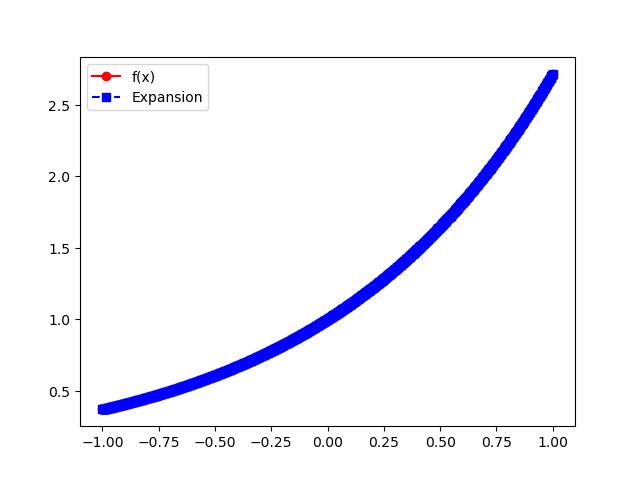
\includegraphics[width=0.49\textwidth]{ex_val.png}
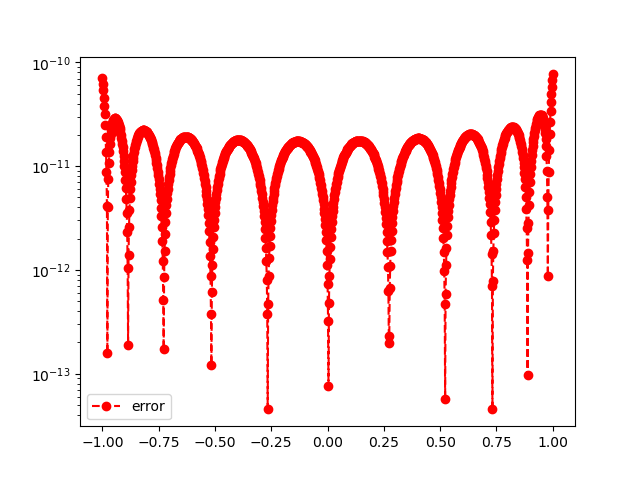
\includegraphics[width=0.49\textwidth]{ex_err.png}

We now approximate the function \begin{align*}
    f(x) = \frac{1}{1+x^2},
\end{align*} with results for \(n=10\) shown below.

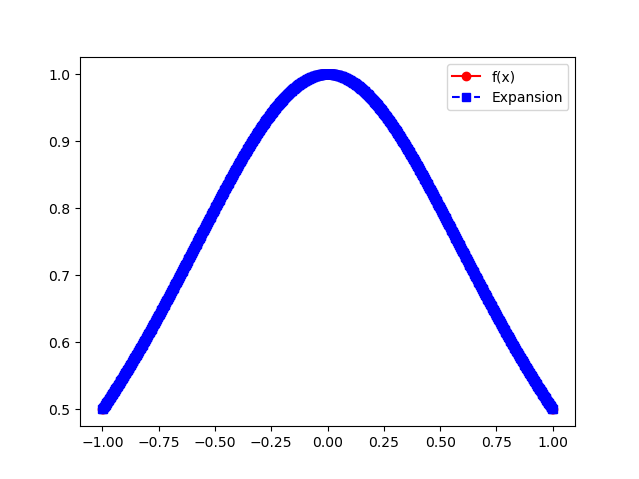
\includegraphics[width=0.49\textwidth]{2_val.png}
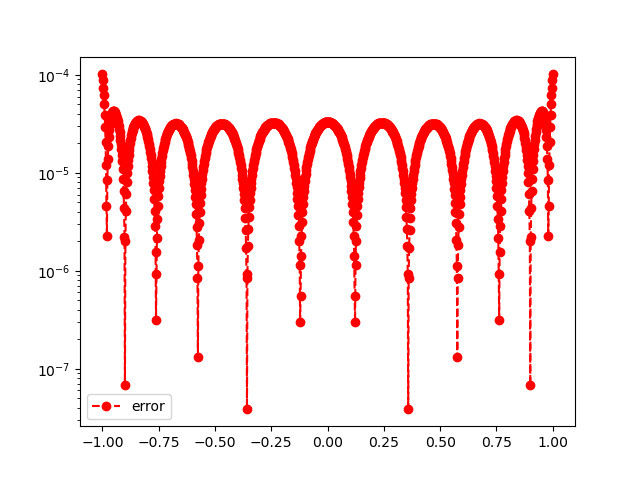
\includegraphics[width=0.49\textwidth]{2_err.png}


{\small \lstinputlisting[language=Python]{lab10.py}}    

\end{document}
